%xelatex -shell-escape -output-directory=bin ergasia.tex
\documentclass{assignment}

\usepackage{enumerate} % Για την χρησιμοποίηση roman enumerate
\usepackage{paralist} % για το περιβάλλον inparaenum που είναι οι λίστες μέσα στο κείμενο.
\usepackage{program}
\usepackage{algorithm}

\title{Αναγνώριση Προτύπων \\ Θέμα Εξαμήνου }
\date{Αθήνα, 2014}

\author{Αναγνωστόπουλος Βασίλης - Θάνος (ΜΠΠΛ 13002) \and Βελισσαρίου Κυριάκος (ΜΠΠΛ 13005)}

\begin{document}

\maketitle
% Να σκεφτώ τί αλλαγές θέλω να κάνω με τις αριθμήσεις και άμα θέλω να κάνω.
% Να σκεφτώ να τις ενσωματώσω και στο assignment.cls

\setcounter{page}{1} 
\pagenumbering{roman}

\pagestyle{plain}
\tableofcontents
%\listoftables
\listoffigures

\makeatletter
\newcommand{\newalgname}[1]{%
  \renewcommand{\ALG@name}{#1}%
}
\newalgname{Αλγόριθμος}
\renewcommand{\listalgorithmname}{Κατάλογος αλγορίθμων}
\makeatother

\listofalgorithms

\renewcommand\listoflistingscaption{Κατάλογος πηγαίου κώδικα}
\renewcommand\listingscaption{Πηγαίος κώδικας}

\listoflistings
\newpage

%\pagestyle{headings}
%\pagestyle{fancy}
\setcounter{page}{1} 
\pagenumbering{arabic}

\section{Άσκηση 1η - \en{Artificial Immune System}}
\subsection{Εκφώνηση}

Να γίνει πλήρης βιβλιογραφική έρευνα με βάση τις λέξεις κλειδιά "\en{Artificial Immune System}".

\subsection {Λύση}

Το φυσικό ανοσοποιητικό σύστημα είναι ένα πολύπλοκο σύστημα για την λειτουργία του οποίου έχουν γραφτεί αρκετές δημοσιεύσεις για το πως λειτουργεί \cite{wiki:immune_system}. Εκτός από την ικανότητα του να καταπολεμά ξένα κύτταρα και μολύνσεις προς τον οργανισμό, διαθέτει μνήμη, μία ιδιαίτερα σημαντική ιδιότητα, καθ` ότι του επιτρέπει να αναγνωρίζει και να αντιμετωπίζει πιο άμεσα σε μία εισβολή από παθογόνα, που έχουν προσβάλει και παλιότερα τον οργανισμό. 

Ένα τεχνητό ανοσοποιητικό σύστημα (ΤΑΣ - αγγλ. \en{Artificial Immune System}) μοντελοποιεί την ικανότητα του φυσικού ανοσοποιητικού συστήματος των σπονδυλωτών να ανιχνεύει κύτταρα ξένα προς τον οργανισμό.Το αποτέλεσμα είναι ένα νέο υπολογιστικό μοντέλο το οποίο είναι ικανό να αναγνωρίζει πρότυπα και εφαρμόζεται κυρίως στην ανίχνευση ανωμαλιών \cite{engelbrecht,wiki:artificial_immune_system}.

Ο ορισμός και η ανάπτυξη ενός πλήρους ΤΑΣ περιλαμβάνει, γενικά, μία πληθώρα θεμάτων, μεταξύ των οποίων είναι \cite{engelbrecht,karakasis_thesis}:

\begin{itemize}
\item υβριδικές δομές και αλγόριθμοι, οι οποίοι λαμβάνουν υπ` υπόψιν τους μηχανισμούς του ανοσοποιητικού συστήματος όπως την ανίχνευση ξένων προτύπων με μία ορισμένη συγγένεια και την αποθήκευση πληροφορίας και την επαναχρησιμοποίηση της.
\item υπολογιστικοί αλγόριθμοι βασισμένοι σε αρχές του ανοσοποιητικού συστήματος, όπως είναι η κατανεμημένη επεξεργασία, η αρχή της επιλογής των κλώνων και η θεωρία του ανοσοποιητικού δικτύου.
\end{itemize}


Χρησιμοποιώντας τα παραπάνω ο \citeauthor{engelbrecht} παραθέτει τον βασικό αλγόριθμο για την δημιουργία ΤΑΣ (βλέπε αλγόριθμο \ref{algorith:AIS}). 
\begin{algorithm}                        % enter the algorithm environment
\caption{Βασικός αλγόριθμος ΤΑΣ \cite{engelbrecht}}          % give the algorithm a caption
\label{algorith:AIS}                      % and a label for \ref{} commands later in the document
\begin{program}
\mbox{Αρχικοποίηση ενός σύνολου τεχνικών λεμφοκυττάρων (ΤΛ) ως πληθυσμός }C;
\mbox{Καθορισμός των προτύπων των αντιγόνων ως σύνολο εκπαίδευσης }D_T;
\WHILE \mbox{κάποια συνθήκη τερματισμού είναι αναληθείς} \DO 
  \FOR \mbox{κάθε πρότυπο αντιγόνου } z_p \in D_T \DO
    \mbox{Επιλογή ενός υποσυνόλου ΤΛ για έκθεση στο }z_p \mbox{,σαν πληθυσμός } S \leq C;
    \FOR \mbox{για κάθε ΤΛ } x_i \in S \DO
          \mbox{Υπολογισμός την ομοιότητα του αντιγόνου μεταξύ } z_p,x_i ;
    \END
    \mbox{Επιλογή ενός υποσυνόλου ΤΛ που έχουν την μεγαλύτερη ομοιότητα }
    \mbox{αντιγόνων σαν πληθυσμός } H \leq S;
    \mbox{Προσαρμογή των ΤΛ με κάποια μέθοδο επιλογής, με βάση την υπολογισμένη}
    \mbox{ομοιότητα και/ή την ομοιότητα του δικτύου των ΤΛ στο }H;
    \mbox{Ανανέωση του βαθμού ομοιότητας των ΤΛ στο }H;
  \END
\END
\end{program}
\end{algorithm}

Κάθε κομμάτι του αλγορίθμου αναλύεται πιο κάτω \cite{engelbrecht}:
\begin{description}
\item[Αρχικοποίηση $C$ και καθορισμός $D_T$:] Ο πληθυσμός $C$ μπορεί να είναι είτε δημιουργημένος από τυχαία δημιουργημένα τεχνητά λεμφοκυττάρων \footnote{Το λεμφοκύτταρο αποτελεί είδος λευκού αιμοσφαιρίου το οποίο το συναντιόνται στο φυσικό ανοσοποιητικό σύστημα και είναι επιφορτισμένα με την άμυνα του οργανισμού έναντι σε λοιμώξεις \cite{wiki:lymphocytes}.} (ΤΛ) ή από κάποια άλλη μέθοδο η οποία εξαρτάται από τον αγλόριθμο του ΤΑΣ.

\item[Συνθήκη τερματισμού του while:] Στα περισσότερα μοντέλα των ΤΑΣ, η συνθήκη τερματισμού βασίζεται στην σύγκλιση του πληθυσμού των ΤΛ ή από ένα συγκεκριμένο αριθμό επαναλήψεων.

\item[Επιλογή του υποσυνόλου $S$ των ΤΛ:] Το υποσύνολο $S$ μπορεί να είναι ολόκληρο το σύνολο $P$ ή ένα τυχαίος αριθμός ΤΛ από το $P$. 

\item[Υπολογισμός της ομοιότητας του αντιγόνου:] Η ομοιότητα του αντιγόνου (αγγλ. \en{antigen affinity}) είναι η μέτρηση της "συγγένειας" που υπάρχει μεταξύ των ΤΛ και των προτύπων των αντιγόνων. 

\item[Επιλογή του υποσυνόλου $H$ των ΤΛ:] Σε κάποια από τα μοντέλα των ΤΑΣ, η επιλογή της καλύτερης ομοιότητας των ΤΛ βασίζεται σε κάποιο κατώφλι ομοιότητας. Έτσι το υποσύνολο $H$ μπορεί να είναι ολόκληρο το $S$, αναλόγως ποιο είναι το κατώφλι ομοιότητας.

\item[Υπολογισμός της ομοιότητας του δικτύου:] Αυτή είναι η μέτρηση της ομοιότητας μεταξύ δύο ΤΛ. Τα διάφορα μέτρα ομοιότητας ενός δικτύου είναι τα ίδια με εκείνα των αντιγόνων.. Ένα καθορισμένο κατώφλι ομοιότητας προσδιορίζει αν δύο ή περισσότερα ΤΛ συνδέονται για να σχηματίσουν ένα δίκτυο.

\item[Ανανέωση του βαθμού ομοιότητας των ΤΛ στο $H$:] Είναι η διαδικασία με την οποία τα ΤΛ ωριμάζουν. Η διαδικασία ωρίμανσης αλλάζει ανάλογα με το μοντέλο του ΤΑΣ.

\end{description}

Έχουν προταθεί αρκετοί αλγόριθμοι για την επίλυση των ΤΑΣ όπως \cite{engelbrecht}:
\begin{description}

\item[το κλασσικό μοντέλο:] σε αυτό το μοντέλο το ΤΑΣ "εκπαιδεύει" τα ΤΛ σε ένα σύνολο προτύπων του εαυτού του έτσι ώστε να είναι "αυτο-ανεκτικά", δηλαδή να έχουν την ικανότητα να αναγνωρίζουν τα πρότυπα μεταξύ του εαυτού και του μη εαυτού \cite{engelbrecht}. Βασίζεται στα Τ-λεμφοκύτταρα του φυσικού ανοσοποιητικού συστήματος τα οποία αναγνωρίζουν τα κύτταρα του οργανισμού και επιτίθενται μόνο στα ξένα κύτταρα. Ένα από τα μοντέλα των ΤΑΣ που βασίζονται στο κλασσικό μοντέλο είναι το μοντέλο της αρνητικής επιλογής.

\item[το μοντέλο επιλογής του κλώνου:]  σε αυτό το μοντέλο των ΤΑΣ η επιλογή ενός συνόλου ΤΛ γίνεται με βάση εκείνα τα οποία έχουν τον υψηλότερο βαθμό ομοιότητας μαζί με ένα πρότυπο μη εαυτού. Έπειτα τα επιλεγμένα ΤΛ κλωνοποιούνται και μεταλλάσσονται σε μία προσπάθεια να έχουν υψηλότερη ομοιότητα με το πρότυπο μη εαυτού.

\item[το μοντέλου του δικτύου:] σε αυτό το μοντέλο των ΤΑΣ τα ΤΛ αλληλεπιδρούν μεταξύ τους έτσι ώστε να μάθει το ένα από το άλλο την μορφή του προτύπου μη εαυτού, με αποτέλεσμα να δημιουργείται ένα δίκτυο από ΤΛ.

\item[το μοντέλο του κινδύνου:] σε αυτό το μοντέλο, σε αντίθεση με το κλασσικό μοντέλο, το μοντέλο του κινδύνου διαφοροποιείται αναγνωρίζοντας το τί είναι επικίνδυνο και τί είναι μη-επικίνδυνο αντί να βρίσκει πρότυπα εαυτού και μη-εαυτού.

\end{description}

Τα τεχνητά ανοσοποιητικά συστήματα έχουν εφαρμοστεί με επιτυχία σε πολλές περιοχές, όπως στην ανίχνευση ανωμαλιών, στην ταξινόμηση δεδομένων, στην ανίχνευση ιών, στην αναγνώριση προτύπων κ.λ.π. \cite{wiki:artificial_immune_system, engelbrecht, karakasis_thesis}.

\section{Άσκηση 2η - Swarm Intelligence}
\subsection{Εκφώνηση}

Να γίνει πλήρης βιβλιογραφική έρευνα με βάση τις λέξεις κλειδιά "\en{Swarm Intelligence}".

\subsection {Λύση}
\subsubsection{Εισαγωγή}
Στην παρούσα ερώτηση θα επιχειρηθεί μια σύντομη έκθεση η οποία θα αφορά τον όρο
Νοημοσύνη Σμήνους (Swarm Intelligence). Η δομή που ακολουθείται είναι η
εξής: Αρχικά, θα δοθεί ο ορισμός της Νοημοσύνης Σμήνους και θα αναφερθούν οι
γενικές αρχές της. Στην συνέχεια, θα γίνει μια σύντομη επισκόπηση στις
κατηγορίες αλγορίθμων νοημοσύνης σμήνους. Τέλος, στον επίλογο, θα αναφερθούν
μια σειρά από προβλήματα, στην επίλυση των οποίων βρίσκουν εφαρμογή οι
προαναφερθέντες αλγόριθμοι.
\subsubsection{Ορισμός - Αρχές}
Σύμφωνα με τους Gerardo Beni και Jim Wang \cite{beni1993swarm}, η Νοημοσύνη
Σμήνους είναι η συλλογική συμπεριφορά αποκεντρωμένων αυτο-οργανωμένων
συστημάτων, φυσικών ή τεχνητών.

Όπως είναι προφανές, τα φυσικά συστήματα νοημοσύνης σμήνους προϋπήρχαν των
τεχνιτών και μάλιστα, στάθηκαν η αφορμή για την δημιουργία των τελευταίων. Τα
φυσικά συστήματα που μελετήθηκαν αρχικά περιελάμβαναν κοπάδια ψαριών, σμήνη
πτηνών και μελισσών καθώς και αποικίες μυρμηγκιών. Αυτό το οποίο εντυπωσίασε
του ερευνητές και που προσπάθησαν να εκμεταλλευτούν με την δημιουργία τεχνητών
συστημάτων νοημοσύνης σμήνους, είναι η δυνατότητα των συστημάτων αυτών, να
πετυχαίνουν πολύπλοκους στόχους ενώ τα ίδια είναι αποτελούμενα από απλές
οντότητες περιορισμένων δυνατοτήτων. Ένα ακόμα εντυπωσιακό στοιχείο, σύμφωνα
και με τον ορισμό που δόθηκε, είναι ότι οι απλές αυτές οντότητες δεν
κατευθύνονται από κάποια κεντρική οντότητα \cite{ahmed2012swarm}, αλλά δρουν
αποκεντρωμένα. Για παράδειγμα, στις αποικίες μυρμηγκιών, τα μυρμήγκια είναι
ικανά όχι μόνο να βρουν τον δρόμο, αλλά και το συντομότερο μονοπάτι προς την
τροφή τους. Αυτό το πετυχαίνουν με την έκκριση μια φερορμόνης. Συνεπώς, τα
μυρμήγκια θα ακολουθούν μονοπάτια τα οποία έχουν έντονη ποσότητα φερορμόνης
για να τα διεγείρει. Τελικά, το συντομότερο μονοπάτι προς την τροφή θα
συγκεντρώνει όλο και μεγαλύτερο αριθμό μυρμηγκιών, έτσι η φερορμόνη σε αυτό το
μονοπάτι θα είναι εντονότερη κοκ \cite{dorigo2006ant}.

Στο επόμενο υποκεφάλαιο παρουσιάζονται κάποιοι από τους σημαντικότερους
αλγόριθμους Νοημοσύνης Σμήνους οι οποίοι προήλθαν από μελέτη φαινομένων σαν
αυτά που αναφέρθηκαν στην προηγούμενη παράγραφο.
\subsubsection{Κυριότεροι αλγόριθμοι σμήνους}
\subsubsection*{Αλγόριθμος PSO}
O αλγόριθμος PSO είναι εμπνευσμένος από τον τρόπο με τον οποίο λειτουργούν
τα σμήνη πουλιών και μελισσών για να προσανατολιστούν στον χώρο. Πρόκειται για
μεταευριστικό αλγόριθμο καθώς δεν κάνει υποθέσεις σχετικά με το πρόβλημα που
πρόκειται να επιλυθεί. Οι αρχική σύλληψη του αλγορίθμου αποδίδεται στον \citet{kennedy2010particle}.

Ο αλγόριθμος βρίσκει πεδίο εφαρμογής σε προβλήματα βελτιστοποίησης τα οποία
έχουν μεγάλους χώρους πιθανών λύσεων. Ωστόσο, ο PSO δεν εγγυάται την εύρεση
της βέλτιστης λύσης, αλλά μια πολύ καλή προσσέγιση αυτής. Το γεγονός της εύκολής
υλοποίησής του σε συνδιασμό με το ότι δεν απαιτεί το πρόβλημα προς
βελτιστοποίηση να είναι παραγωγίσιμο \cite{kennedy2010particle} τον καθιστά μια
καλή επιλογή για προβλήματα που μεταβάλλονται στον χρόνο ή ενέχουν θόρυβο.

Ο αλγόριθμος PSO υπάρχει σε πολλές παραλλαγές, ωστόσο η κύρια μορφή του είναι
αυτή κατά την οποία αναζητείται το ολικό μέγιστο. Επιπλέον, σε ότι αφορά την
τοπολογία του σμήνους, έχουμε ένα πλήρως συνδεδεμένο σμήνος, δηλαδή κάθε μέλος
του σμήνους γνωρίζει τις διαθέσιμες πληροφορίες για όλα τα υπόλοιπα μέλη.
\begin{algorithm}                        % enter the algorithm environment
\caption{Ψευδοκώδικας αλγόριθμου pso}          % give the algorithm a caption
\label{algorith:PSO}                      % and a label for \ref{} commands later in the document
\begin{program}
\mbox{//Αρχικοποίηση};
  \FOR \mbox{κάθε σωματίδιο } i \in S \DO
    \FOR \mbox{κάθε διάσταση } d \in D \DO
    \mbox{//Αρχικοποίηση της ταχύτητας και της θέσης των σωματιδίων}
    x_{i, d} = Rnd(x_{min}, x_{max})
    u_{i,d} = Rnd(-u_{max/3}, u_{max}/3)
    \END
    \mbox{//Αρχικοποίηση της καλύτερης θέσης κάθε σωματιδίου}
    pb_i = x_i
    \mbox{//Ενημέρωση της καθολικά καλύτερης θέσης}
    \IF f(pb_i) \lt f(gb)
    \THEN gb = pb_i
    \FI
  \END

  \mbox{(Αρχικοποίηση)}
  \WHILE it \lt MAX\_ITERATIONS \DO
    \FOR \mbox{κάθε σωματίδιο } i \in S \DO
    \mbox{//Ενημέρωση της καλύτερης θέσης κάθε σωματιδίου}
    \IF f(x_i) \lt f(pb_i)
    \THEN pb_i = x_i
    \FI
    \mbox{//Ενημέρωση του καθολικού μέγιστου}
    \IF f(pb_i) \lt f(gb)
    \THEN gb = pb_i
    \FI
    \END
    \mbox{//Ενημέρωση της ταχύτητας και της θέσης των σωματιδίων}
    \FOR \mbox{κάθε σωματίδιο } i \in S \DO
        \FOR \mbox{κάθε διάσταση } d \in D \DO
            u_{i, d} = u_{i, d} + C_1 * Rnd(0,1) * [pb_{i, d}-x_{i, d}] + C_2 * Rnd(0, 1) * [gb_d - x_{i, d}]
            x_{i, d} = x{i, d} + u{i, d}
        \END
    \END
    \mbox{//Επόμενη επανάληψη}
    it = it + 1
  \END
  \mbox{επέστρεψε } gb
\end{program}
\end{algorithm}
Στον πίνακα \ref{algorith:PSO} φαίνεται ψευδοκώδικας για τον γενικό αλγόριθμο
PSO όπως αυτός ανακτήθηκε από τον ιστότοπο \cite{web:ist}. Ακολουθεί λεκτική
περιγραφή του αλγορίθμου.

Αρχικά ορίζεται η λειτουργία της αρχικοποίησης του σμήνους. Δηλαδή, για κάθε
σωματίδιο του σμήνους, καθώς και για κάθε συνιστώσα της λύσης δίνεται μια τυχαία
τιμή μέσα στις επιτρεπτές τιμές. Είναι φανερό, ότι οι επιτρεπτές τιμές καθώς και
και οι συνιστώσες στις οποίες έχει αποκωδικοποιηθεί η λύση εξαρτώνται από την
δομή του προβλήματος. Στην συνέχεια αρχικοποιείται η καλύτερη θέση κάθε
σωματιδίου, η οποία είναι η τρέχουσα θέση καθώς ο αλγόριθμος δεν έχει ξεκινήσει.
Τέλος, βρίσκεται το ολικό μέγιστο, δηλαδή η θέση η οποία έχει την μεγαλύτερη
αξία. Η αξία δίνεται από την συνάρτηση f η δομή της οποίας εξαρτάται από την
φύση του προβλήματος.

Αφού γίνει η αρχικοποίηση, ορίζουμε μια καθολική μεταβλητή η οποία δείχνει τον
μέγιστο αριθμό των επαναλήψεων της εκτέλεσης του αλγορίθμου. Σε κάθε μια από
αυτές τις επαναλήψεις γίνονται τα εξής: Για κάθε σωματίδιο ανανεώνεται
η καλύτερή του θέση. Επίσης, ανανεώνεται το ολικό μέγιστο. Στην συνέχεια για
κάθε σωματίδιο και κάθε διάσταση της λύσης υπολογίζεται η νέα ταχύτητα και
η νέα θέση. Η νέα θέση προκύπτει από την προηγούμενη θέση συν την ταχύτητα. Σε
ότι αφορά την ενημέρωση της ταχύτητας αυτή προκύπτει από το άθροισμα
διαφορετικών συστατικών. Το πρώτο προκύπτει από την διαφορά της τρέχουσας θέσης
από την καλύτερη θέση που έχει επισκεφθεί το συγκεκριμένο σωματίδιο. Το δεύτερο
προκύπτει από την διαφορά της τρέχουσας θέσης του σωματιδίου από το ολικό
μέγιστο. Παρατηρούμε ότι και τα δύο παραπάνω είναι πολλαπλασιασμένα από δύο
επιταχυντές $C_1$ και $C_2$ αντίστοιχα, καθώς και από μια στοχαστική μεταβλητή
η οποία λαμβάνει κάθε φορά μια τιμή ανάμεσα στο 0 και το 1. Η χρησιμότητα
της στοχαστικής μεταβλητής έγκειται στην αποφυγή της παγίδευσης του αλγορίθμου
σε τοπικό μέγιστο. To τελευταίο συστατικό της στο άθροισμα είναι η τρέχουσα
ταχύτητα. Τέλος, αυξάνεται ο μετρητής επαναλήψεων κατά 1.

Όταν ολοκληρωθεί ο αριθμός των επαναλήψεων που έχει οριστεί, ο αλγόριθμος
τερματίζει και επιστρέφεται η τιμή που υπάρχει στην μεταβλητή $gb$, η οποία
εκφράζει την καλύτερη λύση που έχει βρεθεί συνολικά.
\subsubsection*{Αλγόριθμος ACO}
Ο αλγόριθμος ACO (Ant Colony Optimization) είναι εμπνευσμένος, όπως αναφέρθηκε
παραπάνω, από τον τρόπο με τον οποίο τα μυρμήγκια βρίσκουν τον συντομότερο δρόμο
προς την τροφή τους χρησιμοποιώντας τις φερομόνες. Δημιουργοί του αλγορίθμου
είναι οι \citet{dorigo2010ant}. H κυριότερη εφαρμογή του αλγόριθμου ACO
βρίσκεται σε προβλήματα συνδυαστικής φύσης και πιο συγκεκριμένα σε εύρεση
βέλτιστων μονοπατιών σε γράφους.

Σε μια πραγματική αποικία μυρμηγκιών, εάν ένα σύντομο μονοπάτι προς τροφή έχει
βρεθεί με την διαδικασία που περιγράφηκε παραπάνω, τότε η πλειοψηφία των
μυρμηγκιών θα κινείται σε αυτό. Εάν η τροφή τελειώσει τότε θα αρχίσουν να 
αναζητούνται άλλα μονοπάτια, δηλαδή άλλη βέλτιστη λύση και καθώς θα γίνεται
αυτό οι φερομόνες στο προηγούμενο μονοπάτι θα εξασθενούν προσελκύοντας όλο και
λιγότερα μυρμήγκια. Εκμεταλλευόμενος αυτό ακριβώς το χαρακτηριστικό, ο
αλγόριθμος ACO αποδεικνύεται ιδιαίτερα χρήσιμος σε προβλήματα γράφων των οποίων
η τοπολογία αλλάζει δυναμικά στον χρόνο. Στον πίνακα \ref{algorith:ACO}
καθώς και στην παράγραφο που ακολουθεί περιγράφεται η λειτουργία του βασικού
αλγορίθμου. Σημειώνεται πως εκτός από τον βασικό αλγόριθμο, υπάρχουν διάφορες
παραλλαγές του όπως των \citet{merkle2002ant} και των \citet{yaseen2008ant}.
\begin{algorithm}                        % enter the algorithm environment
\caption{Ψευδοκώδικας αλγόριθμου aco}          % give the algorithm a caption
\label{algorith:ACO}                      % and a label for \ref{} commands later in the document
\begin{program}
\mbox{Αρχικοποίηση της ελκυστικότητας t και της ορατότητας n για κάθε κόμβο};
  \WHILE i \lt MaxIterations \DO
    \FOR \mbox{κάθε } ant \in C \DO
    \mbox{Επιλογή, βάσει εξίσωσης, του επόμενο κόμβου μετακίνησης;}
    \mbox{Καταχώρηση του κόμβου στην λίστα επισκεπτόμενων κόμβων του μυρμηγκιού;}
    \mbox{Eπανάληψη μέχρι κάθε μυρμήγκι να έχει κατασκευάσει μια λύση;}
  \END
  \FOR \mbox{κάθε } ant \in C \DO
  \mbox{Ενημέρωση της ελκυστικότητας κάθε κόμβου από την λύση;}
  \END
  \IF lb \mbox{ καλύτερη από } gb
    \THEN gb = lb
   \FI
   i = i + 1;
  \END
\end{program}
\end{algorithm}

Στον αλγόριθμο, όπως αυτός περιγράφεται στον πίνακα \ref{algorith:ACO}\cite{web:ucla15}
συμβαίνουν τα εξής: Αρχικά, για κάθε κόμβο αρχικοποιείται ο βαθμός
ελκυστικότητάς του και η ορατότητά του η οποία είναι ένα είδος μετρικής, συνήθως
η απόσταση. Στην συνέχεια κάθε μυρμήγκι επιλέγει τον επόμενο κόμβο τον οποίο
θα επισκεφθεί προχωρώντας προς την κατασκευή μια πλήρους λύσης. Η επιλογή
γίνεται βάση της εξίσωσης \ref{eq:p_edge}.
\begin{equation}
\label{eq:p_edge}
Prob(choose\_available\_edge) = \frac{\tau(e) \cdot n(e)}{\sum_{} available\_edges(\tau(e') \cdot n(e'))}
\end{equation}

Όπως φαίνεται από την εξίσωση, όσο μεγαλύτερη είναι η τιμή της φερομόνης τόσο
μεγαλύτερη είναι η πιθανότητα να επιλεγεί ο συγκεκριμένος κόμβος. Επίσης η
πιθανότητα επιλογής μεγαλώνει όσο μικρότερη είναι η απόσταση του κόμβου. Από
αυτό συμπεραίνουμε ότι η $n(e)$ εκφράζει το αντίστροφο της απόστασης.

Στην συνέχεια, και αφού όλα τα εικονικά μυρμήγκια έχουν καταλήξει σε κάποια
λύση, για κάθε έναν από τους κόμβους που συμμετέχουν σε αυτή, ενημερώνεται η
τιμή της φερομόνης (μέτρο της ελκυστικότητας του κόμβου) μέσω της εξίσωσης
\ref{eq:desirability}.
\begin{equation}
    \label{eq:desirability}
\tau(e) = \begin{cases} (1 - p) \cdot \tau(e),& \mbox{εάν ο κόμβος δεν έχει επισκεφθεί}  \\ (1 - p) \cdot \tau(e) + \mbox{νέα φερομόνη},& \mbox{εάν ο κόμβος έχει επισκεφθεί} \end{cases}
\end{equation}

Η παράμετρος $p, 0 \lt p \lt 1$ εκφράζει τον ρυθμό εξάτμισης, δηλαδή το πόσο
γρήγορα μειώνεται η επίδραση της φερομόνης. Συνεπώς, όσο μεγαλύτερος είναι ο
αριθμός, τόσο μεγαλύτερος είναι ο ρυθμός εξάτμισης γεγονός που αυξάνει την
προσαρμοστικότητα του συστήματος. Αντίστοιχα στην περίπτωση που το $p$ είναι
μικρό. Ο όρος \emph{νέα φερομόνη} συνήθως αντιστοιχεί σε έναν λόγο της μορφής
$\frac{Q}{lenth\_of\_tour}$, όπου $Q$ μια σταθερά ελκυστικότητας. Ο παρονομαστής
αποτελεί το μέγεθος που κατά περίπτωση θέλουμε να βελτιστοποιήσουμε.

Στην συνέχεια ελέγχεται εάν το τοπικό μέγιστο που έχει βρεθεί αποτελεί καλύτερη
λύση από την καθολική λύση μέχρι εκείνη την στιγμή. Εάν η συνθήκη ισχύει τότε
η καθολική λύση ανανεώνεται. Τέλος, αυξάνεται ο αριθμός των επαναλήψεων κατά
μια.
\subsubsection*{Εφαρμογές Αλγόριθμων Νοημοσύνης Σμήνους}
\section{Άσκηση 3η}
\subsection{Εκφώνηση}

Να γίνει πλήρης βιβλιογραφική έρευνα με βάση τις λέξεις κλειδιά "\en{Evolutionary Computing}" και \en{Genetic Algorithms}.

\subsection {Λύση}

σελ. 80

\section{Άσκηση 4η - \en{Fuzzy Logic Systems}}
\subsection{Εκφώνηση}

Να γίνει πλήρης βιβλιογραφική έρευνα με βάση τις λέξεις κλειδιά "\en{Fuzzy Logic Systems}".

\subsection {Ασαφής Λογική}

Η ασαφής λογική πρόκειται για μία γενίκευση της συμβατικής Θεωρίας Συνόλων και είναι μία πλειότιμη λογική η οποία ασχολείται με την λογική σαν μία προσέγγιση και όχι σαν κάτι σταθερό και ακριβές \cite{engelbrecht,class_notes,wiki:fuzzy_logic,zadeh1994}. %Fuzzy logic is a form of many-valued logic which deals with reasoning that is approximate rather than fixed and exact.

Η ασαφής λογική βασίζεται στα ασαφή σύνολα. Σε σύγκριση με τα δυαδικά σύνολα (οι μεταβλητές των οποίων μπορούν να λάβουν την τιμή "αλήθεια" ή "ψευδές"), τα ασαφή σύνολα περιέχουν αντικείμενα τα οποία ικανοποιούν ανακριβείς ιδιότητες και μπορεί να έχουν μία τιμή αληθείας η οποία κυμαίνεται στο βαθμό μεταξύ 0 και 1 σε αυτό το σύνολο (βλ. εξίσωση \eqref{eq:fuzzy_set}) \cite{zadeh1965338}. 

\begin{equation}
\mu_A : X \rightarrow [0,1]
\label{eq:fuzzy_set}
\end{equation}

όπου $X$ ο χώρος των αντικειμένων. Αν $x$ ένα γενικό αντικείμενο του $X$ με $x \in X$ τότε το $\mu_A(x)$ δείχνει την βεβαιότητα με την οποία το στοιχείο $x$ ανήκει στο ασαφή σύνολο $A$.

Ο βαθμός συμμετοχής σε ένα ασαφές σύνολο υποδηλώνει την βεβαιότητα (ή την αβεβαιότητα) ότι το στοιχείο ανήκει σε αυτή την ομάδα. Η ασαφής λογική χρησιμοποιείται για να χειριστεί την έννοια της μερικής αλήθειας, όπου η τιμή της αλήθειας μπορεί να κυμαίνεται μεταξύ εντελώς αλήθειας και εντελώς ψευδή. Τα ασαφή σύνολα επιτρέπουν την μοντελοποίηση των αβεβαιοτήτων της φυσικής γλώσσας και μπορούν να χρησιμοποιηθούν τόσο για διακριτούς ή/και συνεχόμενους χώρους \cite{engelbrecht,class_notes,wiki:fuzzy_logic}. 

Για τον πλήρη ορισμό ενός ασαφές συνόλου χρειαζόμαστε ακόμα και την συνάρτηση μέλος του ασαφούς συνόλου, η οποία χρησιμοποιείται για να συνδέσει τον βαθμό συμμετοχής κάθε στοιχείου $x$ του χώρου των αντικειμένων με το αντίστοιχο ασαφές σύνολο. Οι συναρτήσεις μέλη μπορεί να έχουν οποιοδήποτε σχήμα ή τύπο (βλ. σχήμα \ref{fig:fuzzy_logic_membership_function}). \cite{engelbrecht}.

\begin{figure}[htbp]
  \centering
  \begin{subfigure}[b]{0.5\textwidth}
     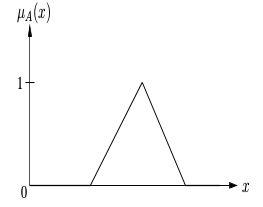
\includegraphics[width=\textwidth,height=0.25\textheight]{images/fuzzy_logic_membership_function_triangular.png}
  \caption{Τριγωνική συνάρτηση μέλους}
  \end{subfigure}%
   ~ %add desired spacing between images, e. g. ~, \quad, \qquad, \hfill etc.
  \begin{subfigure}[b]{0.5\textwidth}
    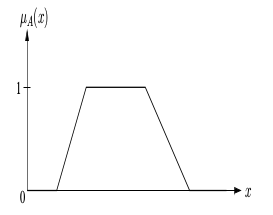
\includegraphics[width=\textwidth,height=0.25\textheight]{images/fuzzy_logic_membership_function_trapezoidal.png}
  \caption{Τραπεζοειδής συνάρτηση μέλους}
  \end{subfigure}
   ~ %add desired spacing between images, e. g. ~, \quad, \qquad, \hfill etc.
  \begin{subfigure}[b]{0.4\textwidth}
    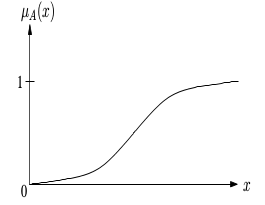
\includegraphics[width=\textwidth,height=0.25\textheight]{images/fuzzy_logic_membership_function_logistic.png}
  \caption{Λογιστική συνάρτηση μέλους}
  \end{subfigure}
   ~ %add desired spacing between images, e. g. ~, \quad, \qquad, \hfill etc.
  \begin{subfigure}[b]{0.5\textwidth}
    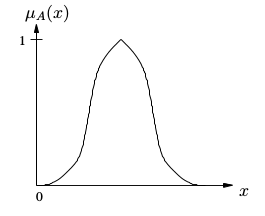
\includegraphics[width=\textwidth,height=0.25\textheight]{images/fuzzy_logic_membership_function_gaussian.png}
  \caption{Γκαουσιανή συνάρτηση μέλους}
  \end{subfigure}
  \caption{Παραδείγματα συναρτήσεων μελών \cite{engelbrecht}}
\label{fig:fuzzy_logic_membership_function}
\end{figure}

Τέλος στην ασαφή λογική μπορούν να χρησιμοποιηθούν και λεκτικές μεταβλητές (αγγλ. \en{linguistic variables}). Με τον όρο λεκτική μεταβλητή εννοούμε τις μεταβλητές των οποίων οι τιμές είναι λέξεις σε μία φυσική ή τεχνική γλώσσα \cite{zadeh1975concept}. Οι λεκτικές μεταβλητές επιτρέπουν την μετατροπή της φυσικής γλώσσας σε λογικές ή αριθμητικές παραστάσεις, οι οποίες παρέχουν τα εργαλεία για την προσεγγιστική λογική \cite{engelbrecht}.

\subsection{Συστήματα ασαφούς λογικής}

Η σχεδίαση συστημάτων ασαφούς λογικής (ΣΑΛ) είναι ένας από τους μεγαλύτερους τομείς εφαρμογής της ασαφούς λογικής \cite{engelbrecht}. Ένα σύστημα ασαφούς λογικής (αγγλ. \en{Fuzzy Logic Systems - FLS}) είναι μία γραμμική απεικόνιση ενός διανύσματος δεδομένων εισόδου (χαρακτηριστικά) σε μία βαθμωτή έξοδο (η οποία αποσυντίθεται σε μία συλλογή από ανεξάρτητες πολλαπλές εισόδου/μονής εξόδου σύστημα - βλέπε σχήμα \ref{fig:fuzzy_logic_system}) \cite{mendel364485,class_notes}.

\begin{figure}
\begin{center}
\resizebox*{\textwidth}{!}{
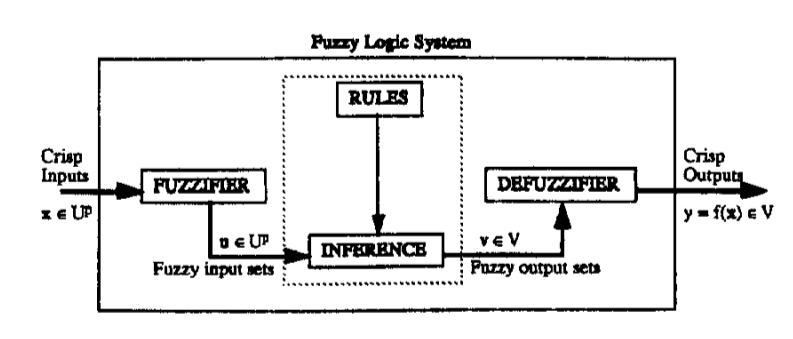
\includegraphics{images/fuzzy_logic_system.png}}
\caption{Σύστημα ασαφούς λογικής \cite{mendel364485,class_notes}}
\label{fig:fuzzy_logic_system}
\end{center}
\end{figure}

Στα ΣΑΛ, η δυναμική συμπεριφορά του συστήματος περιγράφεται από ένα σύνολο λεκτικών ασαφών κανόνων της μορφής ΑΝ - ΤΟΤΕ \cite{engelbrecht, class_notes}. Σε συνδυασμό, τα ασαφή σύνολα και οι λεκτικοί κανόνες αποτελούν την γνωσιακή βάση ενός ΣΑΛ. Ακόμα ένα ΣΑΛ αποτελείται από άλλα 3 
στοιχεία:

\begin{description}
\item[ασαφοποιητής (αγγλ. \en{fuzzifier}): ] ο σκοπός του ασαφοποιητή είναι η εύρεση μίας ασαφούς τιμής από μη ασαφές τιμές εισόδου. Αυτό επιτυχάνεται χρησιμοποιώντας την συνάρτηση μέλους που σχετίζεται με κάθε ασαφές σύνολο στα δεδομένα εισόδου. Δηλαδή, οι τιμές στα δεδομένα εισόδου αντιστοιχούνται σε βαθμούς συμμετοχής σε ασαφή σύνολα \cite{engelbrecht}.

\item [συμπερασματοποιητής (αγγλ. \en{inference}): ] o σκοπός του συμπερασματοποιητή (αγγλ. \en{inference}) είναι να χαρτογραφήσει τις ασαφές εισόδους (όπως λαμβάνονται από την διαδικασία της ασαφοποίησης (αγγλ. \en{fuzzifier}) στους λεκτικούς κανόνες και να παράγουν μία αποσαφηνισμένη (αγγλ. \en{fuzzified}) έξοδο για κάθε κανόνα \cite{engelbrecht}.

\item [αποσαφηνιστής(αγγλ. \en{defuzzifier}): ] ο σκοπός του αποσαφηνιστή (αγγλ. \en{defuzzifier}) είναι η παραγωγή μίας σαφούς εξόδους για το ΣΑΛ από το ασαφές σύνολο που προέκυψε ως έξοδος από τον συμπερασματοποιητή. Δηλαδή παραγάγει σε αυτό το στάδιο γίνεται η μετατροπή των ασαφών κανόνων σε μία βαθμωτή τιμή ή γενικά σε μή ασαφή μεταβλητή \cite{class_notes,engelbrecht}. Στην βιβλιογραφία έχουν προταθεί αρκετοί αποσαφηνιστές για την εύρεση της βαθμωτής τιμής που αναπαριστά την ενέργεια που πρέπει να πραγματοποιηθεί.
\end{description}

Καθένα από αυτά τα στοιχεία εκτελεί μία συγκεκριμένη εργασία κατά την διαδικασία συλλογισμού (αγγλ. \en{reasoning process}). Τα διαφορετικά στοιχεία ενός ΣΑΛ φαίνονται στο σχήμα \ref{fig:fuzzy_logic_system_2}.

\begin{figure}
\begin{center}
\resizebox*{\textwidth}{!}{
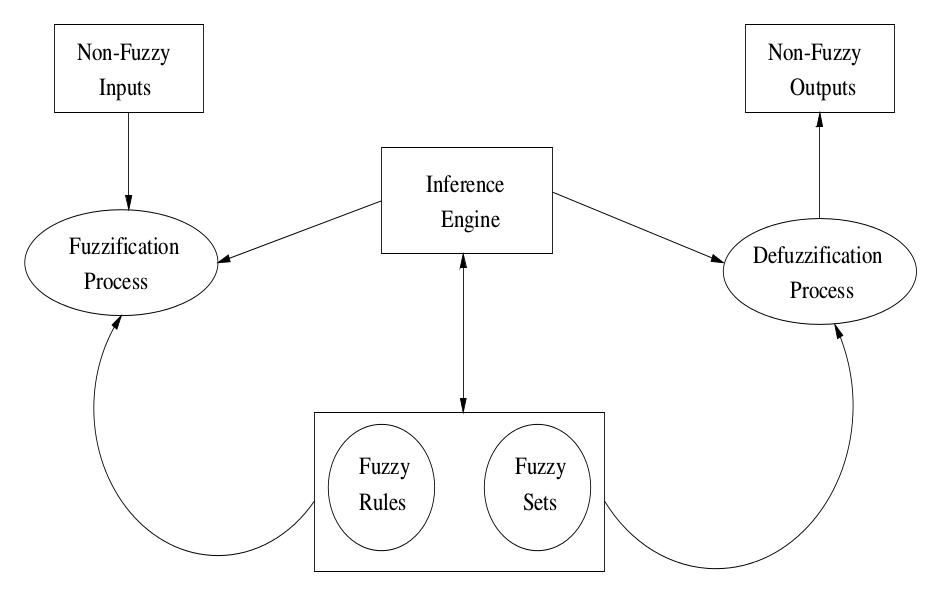
\includegraphics{images/fuzzy_logic_system_2.png}}
\caption{Σύστημα ασαφούς λογικής (2) \cite{engelbrecht}}
\label{fig:fuzzy_logic_system_2}
\end{center}
\end{figure}


\section{Άσκηση 5η}
\subsection{Εκφώνηση}

Να υλοποιηθούν αλγόριθμοι ιεραρχικής ομαδοποίησης δεδομένων και να εφαρμοστούν στα δεδομένα εκφράσεων προσώπου που θα σας παρασχεθούν.

\subsection {Λύση}

Η ιεραρχική ομαδοποίηση (αγγλ. \en{hierarchical clustering}) είναι μία μέθοδος ανάλυσης κλάσεων η οποία αναζητά να κατασκευάσει μία ιεραρχία ομάδων. Η ιεραρχική ομαδοποίηση έχει την ιδιότητα ότι τα δείγματα που ανήκουν στην ίδια ομάδα σε κάποιο επίπεδο να παραμένουν στην ίδια ομάδα σε υψηλότερα επίπεδα \cite{wiki:hierarchical_clustering, class_notes}.

Οι στρατηγικές ιεραρχικής ομαδοποίησης διακρίνονται σε δύο κατηγορίες \cite{wiki:hierarchical_clustering, class_notes}:
\begin{description}
\item[συγχωνευτικές (αγγλ. \en{agglomerative}):] Οι συγχωνευτικές (από κάτω προς τα πάνω) ξεκινούν από $n$ ομάδες και δημιουργούν μία ακολουθία από διαδοχικές συγχωνεύσεις ομάδων.
\item[διαιρετικές (αγγλ. \en{divisive}):]  Οι διαιρετικές (από πάνω προς τα κάτω) ξεκινούν με όλα τα δείγματα σε μία ομάδα και δημιουργούν μία ακολουθία από διαδοχικές διαιρέσεις ομάδων.
\end{description}
 
Τα αποτελέσματα της ιεραρχική ομαδοποίηση συνήθως απεικονίζονται σε ένα δενδρόγραμμα (αγγλ. \en{dendogram}).

Για να διαπιστωθεί ποιες ομάδες θα πρέπει να συγχωνευτούν (ή αντιστοίχως να διαιρεθούν), θα πρέπει να υπάρχει ένα μέτρο της ανομοιότητας μεταξύ των ομάδων των παρατηρήσεων. Στην πλειοψηφία των ιεραρχικών ομαδοποιήσεων αυτό επιτυγχάνετε με την χρήση ενός κατάλληλου μέτρου (ένα μέτρο της απόστασης μεταξύ των ζευγών των παρατηρήσεων - βλ. πίνακα \ref{table:metric_distances}), καθώς και ένα κριτήριο συνδέσεως (βλ. πίνακα \ref{table:metric_linkage}) η οποία καθορίζει την ανομοιότητα των συνόλων ως συνάρτηση των αποστάσεων κατά ζεύγη των παρατηρήσεων στα σύνολα \cite{wiki:hierarchical_clustering}.

\begin{table}[htbp]
\begin{center}
  \begin{tabular}{|m{0.35\textwidth}|m{0.6\textwidth}|}
    \hline
    {\bf Όνομα} & {\bf Τύπος}  \\ \hline
    Ευκλείδια απόσταση   & $\|a-b \|_2 = \sqrt{\sum_i (a_i-b_i)^2}$  \\ \hline
    Απόσταση manhattan   & $\|a-b \|_1 = \sum_i \|a_i-b_i \|$ \\ \hline
    Μέγιστη απόσταση     & $\|a-b \|_\infty = \max_i \|a_i-b_i\|$ \\ \hline
    Απόσταση mahalanobis & $ \sqrt{(a-b)^{\top}S^{-1}(a-b)} $, όπου $S$ είνια ο πίνακας συμεταβλητότητας   \\ \hline
  \end{tabular}
\caption{Ο πίνακας με τις αποστάσεις \cite{wiki:hierarchical_clustering}.}
\label{table:metric_distances}
\end{center}
\end{table}


\begin{table}[htbp]
\begin{center}
  \begin{tabular}{|m{0.35\textwidth}|m{0.6\textwidth}|}
    \hline
    {\bf Όνομα} & {\bf Τύπος}  \\ \hline
    Πλήρης σύνδεσης   & $\max \, \{\, d(a,b) : a \in A,\, b \in B \,\}$  \\ \hline
    Μονή σύνδεση   & $ \min \, \{\, d(a,b) : a \in A,\, b \in B \,\}$ \\ \hline
    Μέση σύνδεση   & $\frac{1}{|A| |B|} \sum_{a \in A }\sum_{ b \in B} d(a,b)$ \\ \hline
  \end{tabular}
\caption{Ο πίνακας με τα κριτήρια σύνδεσης \cite{wiki:hierarchical_clustering}.}
\label{table:metric_linkage}
\end{center}
\end{table}


Στον πηγαίο κώδικα \ref{listing:matlab} φαίνεται το script που γράφτηκε για τον υπολογισμό των ιεραρχικών ομαδοποιήσεων στο matlab.

\captionof{listing}{Ο κώδικας του \en{matlab}}
\inputminted[breaklines=true, frame=lines, framesep=2mm, baselinestretch=1.2, fontsize=\footnotesize, linenos]{matlab}{../matlab/features.m} 
\label{listing:matlab}

Στο σχήμα \ref{fig:data_points} φαίνονται τα χαρακτηριστικά όπως είναι ταξινομημένα στην πραγματικότητα και όπως τα αντιλαμβάνεται ο αλγόριθμος.

Για την καλύτερη κατανόηση της επίδρασης του μέτρου της απόστασης (βλ. πίνακα \ref{table:metric_distances}) και της απόστασης μεταξύ των ζευγών παρατηρήσεων (βλ. πίνακα \ref{table:metric_linkage}) πραγματοποιήθηκαν μία σειρά από ιεραρχικές ταξινομήσεις. Στις 3 πρώτες (βλ. σχήμα \ref{fig:clustering_average_euclidean} έως \ref{fig:clustering_average_manhattan}) διατηρήθηκε σταθερή η απόσταση μεταξύ των ζευγών (και συγκεκριμένα μέση σύνδεση) και άλλαζε ο τύπος της απόστασης ενώ στα 2 τελευταία (βλ. σχήμα \ref{fig:clustering_single_euclidean} έως \ref{fig:clustering_complete_euclidean}) διατηρήθηκε ο τύπος της απόστασης σταθερός (και συγκεκριμένα ευκλείδεια) και άλλαζε η απόσταση μεταξύ των ζευγών.

Παρατηρούμε ότι οι συστάδες που δημιουργήθηκαν δεν αλλάξαν παρά μόνο στο σχήμα \ref{fig:clustering_average_mahalanobis}. Άρα οι συστάδες επηρρεάζονται περισσότερο από την γεωμετρία του ίδιου του προβλήματος παρά από τις παραμέτρους που βάζουμε. Αντιθέτως το δενδρόγραμμα άλλαζε κάθε φορά πράγμα που το καθιστά και ευαίσθητο στις παραμέτρους που τοποθετούμε στο πρόβλημα.

\begin{figure}[htbp]
  \centering
  \begin{subfigure}[b]{0.5\textwidth}
     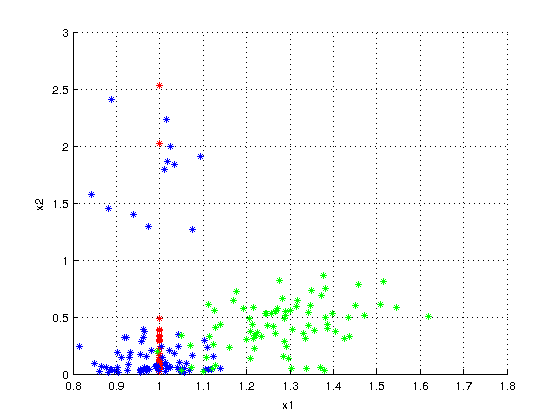
\includegraphics[width=\textwidth,height=0.25\textheight]{matlab/labeled_data_points.png}
  \caption{Τα ταξινομημένα δεδομένα}
  \end{subfigure}%
   ~ %add desired spacing between images, e. g. ~, \quad, \qquad, \hfill etc.
  \begin{subfigure}[b]{0.5\textwidth}
    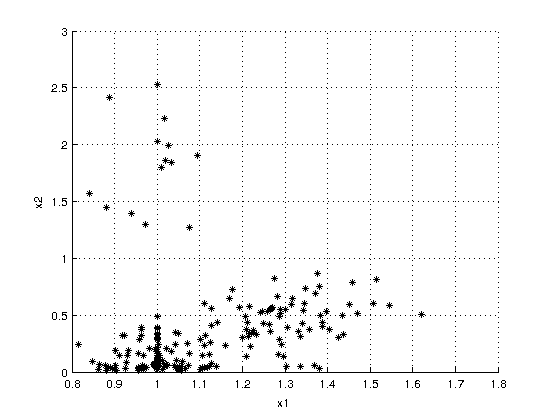
\includegraphics[width=\textwidth,height=0.25\textheight]{matlab/unlabeled_data_points.png}
  \caption{Τα αταξινομημένα δεδομένα}
  \end{subfigure}

  \caption{Τα δεδομένα εκφράσεων προσώπου}
\label{fig:data_points}
\end{figure}

\begin{figure}[htbp]
  \centering
  \begin{subfigure}[b]{0.5\textwidth}
     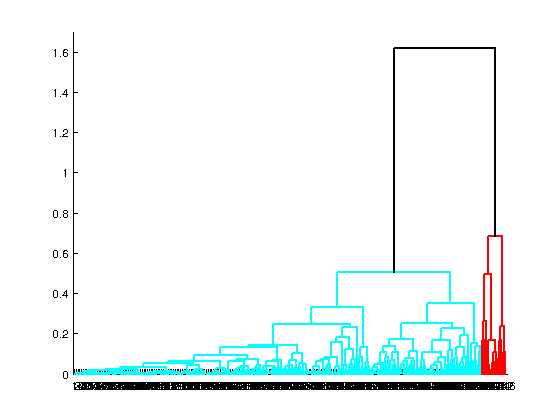
\includegraphics[width=\textwidth,height=0.25\textheight]{matlab/hierarchical_dendogram_average_euclidean.png}
  \caption{Τα δενδρογραμμα των δεδομένα}
  \end{subfigure}%
   ~ %add desired spacing between images, e. g. ~, \quad, \qquad, \hfill etc.
  \begin{subfigure}[b]{0.5\textwidth}
    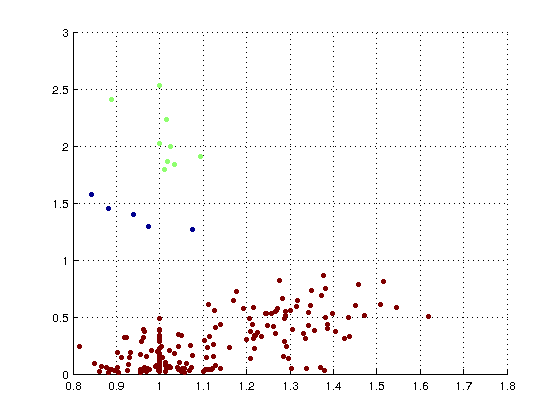
\includegraphics[width=\textwidth,height=0.25\textheight]{matlab/identified_clusters_average_euclidean.png}
  \caption{Οι συστάδες που δημιουργήθηκαν}
  \end{subfigure}

  \caption{Η ιεραρχική ομαδοποίηση των δεδομένων χρησιμοποιώντας την μέση σύνδεση και την ευκλείδεια απόσταση}
\label{fig:clustering_average_euclidean}
\end{figure}

\begin{figure}[htbp]
  \centering
  \begin{subfigure}[b]{0.5\textwidth}
     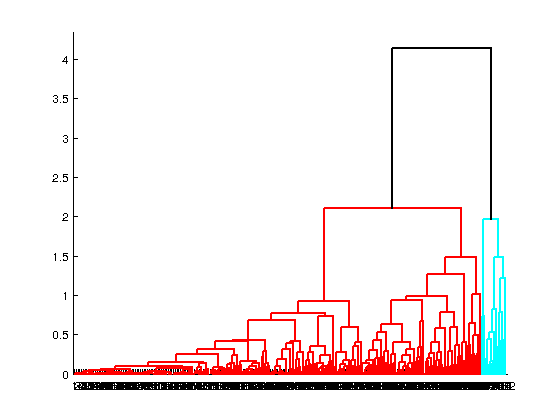
\includegraphics[width=\textwidth,height=0.25\textheight]{matlab/hierarchical_dendogram_average_mahalanobis.png}
  \caption{Τα δενδρογραμμα των δεδομένα}
  \end{subfigure}%
   ~ %add desired spacing between images, e. g. ~, \quad, \qquad, \hfill etc.
  \begin{subfigure}[b]{0.5\textwidth}
    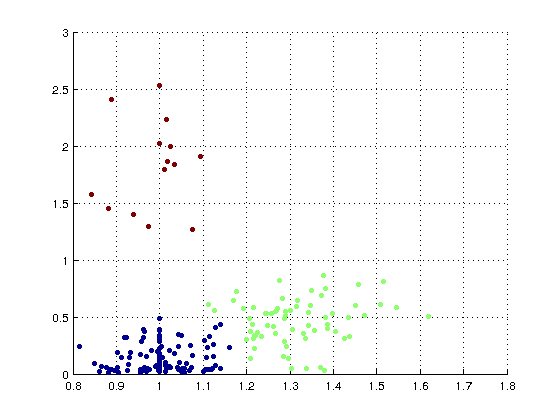
\includegraphics[width=\textwidth,height=0.25\textheight]{matlab/identified_clusters_average_mahalanobis.png}
  \caption{Οι συστάδες που δημιουργήθηκαν}
  \end{subfigure}

  \caption{Η ιεραρχική ομαδοποίηση των δεδομένων χρησιμοποιώντας την μέση σύνδεση και την απόσταση mahalanobis}
\label{fig:clustering_average_mahalanobis}
\end{figure}

\begin{figure}[htbp]
  \centering
  \begin{subfigure}[b]{0.5\textwidth}
     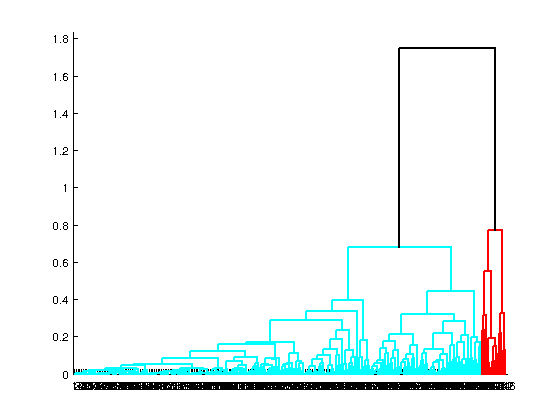
\includegraphics[width=\textwidth,height=0.25\textheight]{matlab/hierarchical_dendogram_average_manhattan.png}
  \caption{Τα δενδρογραμμα των δεδομένα}
  \end{subfigure}%
   ~ %add desired spacing between images, e. g. ~, \quad, \qquad, \hfill etc.
  \begin{subfigure}[b]{0.5\textwidth}
    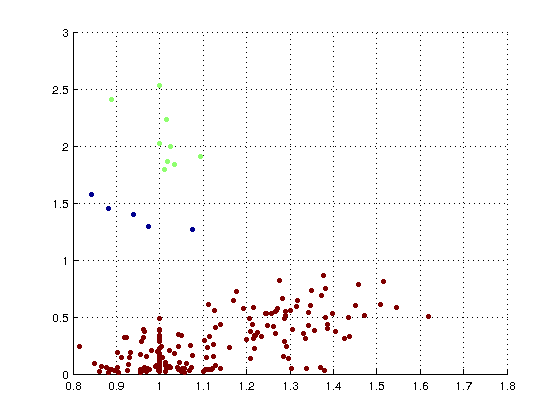
\includegraphics[width=\textwidth,height=0.25\textheight]{matlab/identified_clusters_average_manhattan.png}
  \caption{Οι συστάδες που δημιουργήθηκαν}
  \end{subfigure}
  \caption{Η ιεραρχική ομαδοποίηση των δεδομένων χρησιμοποιώντας την μέση σύνδεση και την απόσταση manhattan}
\label{fig:clustering_average_manhattan}
\end{figure}

\begin{figure}[htbp]
  \centering
  \begin{subfigure}[b]{0.5\textwidth}
     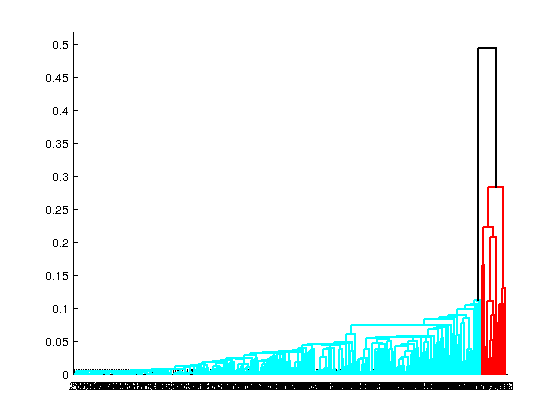
\includegraphics[width=\textwidth,height=0.25\textheight]{matlab/hierarchical_dendogram_single_euclidean.png}
  \caption{Τα δενδρογραμμα των δεδομένα}
  \end{subfigure}%
   ~ %add desired spacing between images, e. g. ~, \quad, \qquad, \hfill etc.
  \begin{subfigure}[b]{0.5\textwidth}
    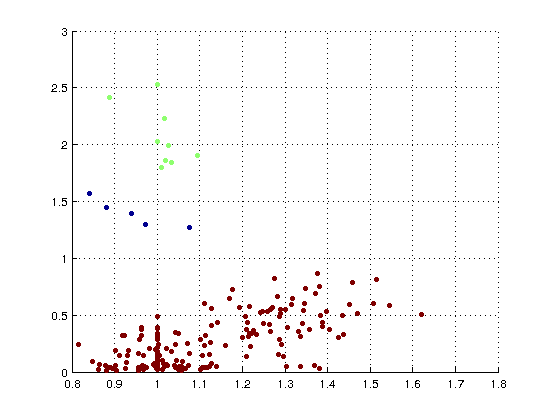
\includegraphics[width=\textwidth,height=0.25\textheight]{matlab/identified_clusters_single_euclidean.png}
  \caption{Οι συστάδες που δημιουργήθηκαν}
  \end{subfigure}
  \caption{Η ιεραρχική ομαδοποίηση των δεδομένων χρησιμοποιώντας την μονή σύνδεση και την ευκλείδεια απόσταση}
\label{fig:clustering_single_euclidean}
\end{figure}

\begin{figure}[htbp]
  \centering
  \begin{subfigure}[b]{0.5\textwidth}
     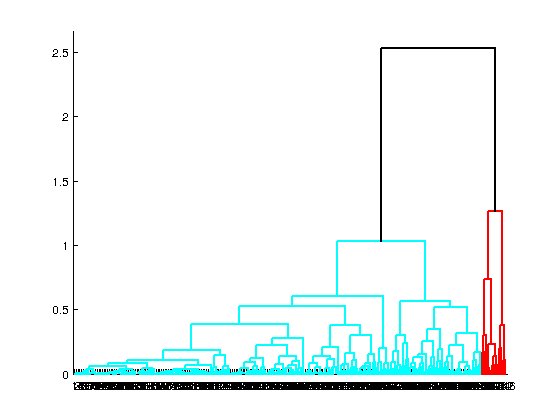
\includegraphics[width=\textwidth,height=0.25\textheight]{matlab/hierarchical_dendogram_complete_euclidean.png}
  \caption{Τα δενδρογραμμα των δεδομένα}
  \end{subfigure}%
   ~ %add desired spacing between images, e. g. ~, \quad, \qquad, \hfill etc.
  \begin{subfigure}[b]{0.5\textwidth}
    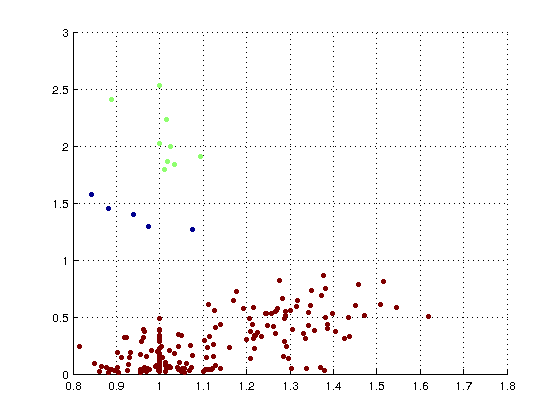
\includegraphics[width=\textwidth,height=0.25\textheight]{matlab/identified_clusters_complete_euclidean.png}
  \caption{Οι συστάδες που δημιουργήθηκαν}
  \end{subfigure}
  \caption{Η ιεραρχική ομαδοποίηση των δεδομένων χρησιμοποιώντας την πλήρη σύνδεση και την ευκλείδεια απόσταση}
\label{fig:clustering_complete_euclidean}
\end{figure}

\clearpage
\phantomsection \label{Βιβλιογραφία}
\addcontentsline{toc}{section}{Βιβλιογραφία}
%\mtcaddchapter[Βιβλιογραφία] % Λόγω του minitoc
\bibliographystyle{plainnat}
\bibliography{references.bib}

\newpage

\end{document}

